\documentclass{article}
\usepackage{hyperref, amsmath, amssymb, tikz, outlines}

\begin{document}
\title{COM2031 EXAM NOTES, CONDENSED}
\author{Jim Lam}
\maketitle

\section{Divide and Conquer}
\subsection{Tiling example}
$2^n$ grid tilings problem

\begin{figure}[htbp]
    \centering
    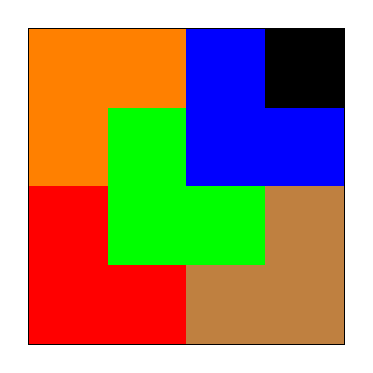
\begin{tikzpicture}[scale=1]
        \draw[step=1cm,gray,very thin] (0,0) grid (4,4);
        \draw[thick] (0,0) rectangle (4,4);
        \fill[orange,opacity=1] (0,2) rectangle (2,4);
        \fill[brown,opacity=1] (2,0) rectangle (4,2);
        \fill[red,opacity=1] (0,0) rectangle (2,2);
        \fill[green,opacity=1] (1,1) rectangle (3,3);
        \fill[blue,opacity=1] (2,2) rectangle (4,4);
        \fill[black,opacity=1] (3,3) rectangle (4,4);
    \end{tikzpicture}
    \caption{Example of a 4x4 grid with some tiles}
\end{figure}

\subsubsection{Base case}
$2^1$ (2x2 grid): 4 ways to tile with L-shape tiles

\subsubsection{Recursive case}
$2^2$: Divide grid into 4 quadrants, tile each quadrant

\subsection{Quicksort}
Brief runthrough (add key points)

\section{Graphs}
\subsection{Graph representation}
\begin{outline}
    \1 Adjacency matrix
    \1 Adjacency list
    \1 Edge list
\end{outline}

\subsection{Graph traversal}
\begin{outline}
    \1 Depth-first search (DFS)
    \1 Breadth-first search (BFS)
\end{outline}

\subsection{Minimum spanning tree}
\begin{outline}
    \1 Kruskal's algorithm
    \1 Prim's algorithm
\end{outline}

\end{document}